\graphicspath{{./figures}}

\section{Ground Station}
A block diagram of the system components for the ground station is shown in Figure \ref{fig:gs_system}.

\begin{figure}[!htb]
  \centering
  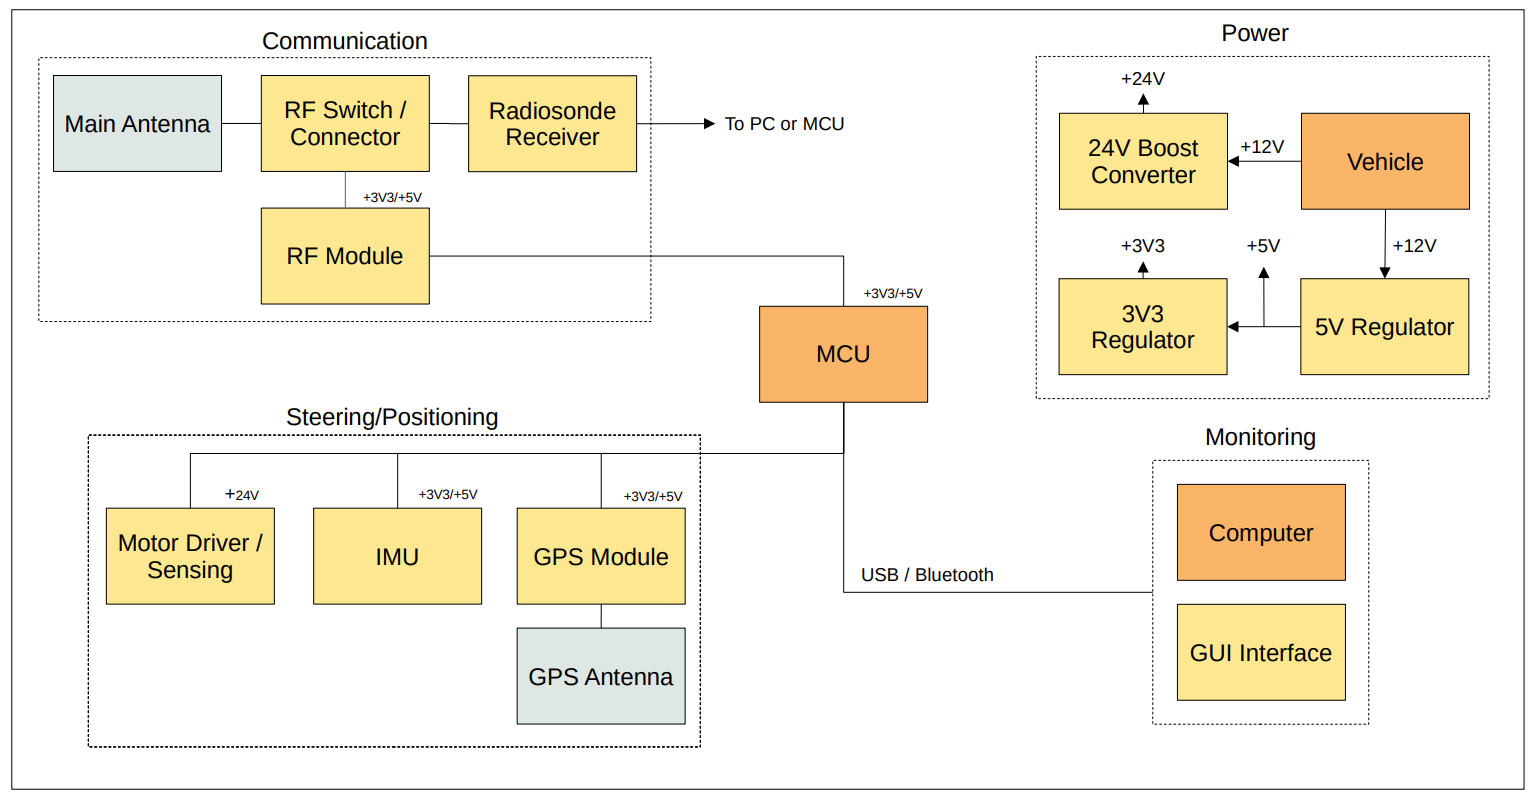
\includegraphics[width=0.95\textwidth]{gs_system}
  \caption{Groud Station System Diagram}
  \label{fig:gs_system}
\end{figure}

\subsection{Power}
The power section consists of two linear regulators, as well as a boost converter. The existing antenna mount has two \textit{NEMA 17 4218S-15} stepper motors, which will be used to steer the ground station in the direction of the satellite. These motors are ideally powered from +24V, and therefore a boost converter will be used to step up the voltage from the car's voltage of +12V. Further, +5V and +3V3 regulators will be ncl to power both the MCU and any other ICs, depending on the voltage level they require.

\subsection{Communication}
The communication section consists of the main antenna, as well as the RF control circuitry and connectors. The \textit{RF Switch/Connector} is provided to allow the antenna to be shared between custom and the proprietary communication protocols. Initially, a connector will be used for prototyping. Then, if time allows, a dedicated RF switch will be included, which will allow for the MCU to control the antenna connection. Both the RF module and the Radiosonde receiver will connect through the RF switch/connector and to the antenna. The Radiosonde will either connect to the PC (if an SDR dongle is used) or to the MCU (if a dedicated receiver is used).

\subsection{Steering and Position}\label{sec:gs_steering_positioning}
\begin{figure}[!htb]
    \centering
    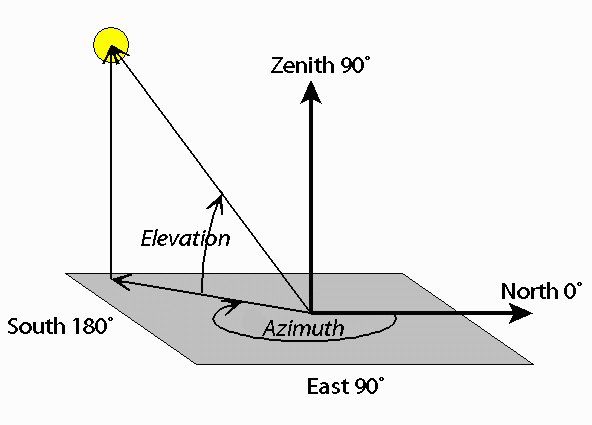
\includegraphics[width=0.4\textwidth]{az_elevation}
    \caption{Azimuthal and Elevation Visualization \cite{site-azElevationVisual}}
    \label{fig:az_elevation}
\end{figure}

Generally, the orientation of the ground station's antenna is described by both an azimuthal and an elevation angle, as in Figure \ref{fig:az_elevation}. The resultant two angles should be controllable to a reasonable degree of accuracy, such that the antenna can point in a given direction.

The existing two-axis antenna mount is shown in Figure \ref{fig:antennaMount}. Since the antenna platform moves relative to the base (where the PCB is mounted), this relative angle needs to be known. Two options to do this are considered:
\begin{enumerate}
    \item \textit{Open-loop}. The base's absolute orientation is measured in realtime, and the platform's relative orientation is pre-computed ("calibrated"); stored in firmware for each combination of stepper motor steps; and looked up in a table when needed.
    \item \textit{Closed-loop}. The platform's itself's absolute orientation is measured in realtime, and this information is fed back into the motor's control system to point the platform correctly.
\end{enumerate}

\begin{figure}[!htb]
    \centering
    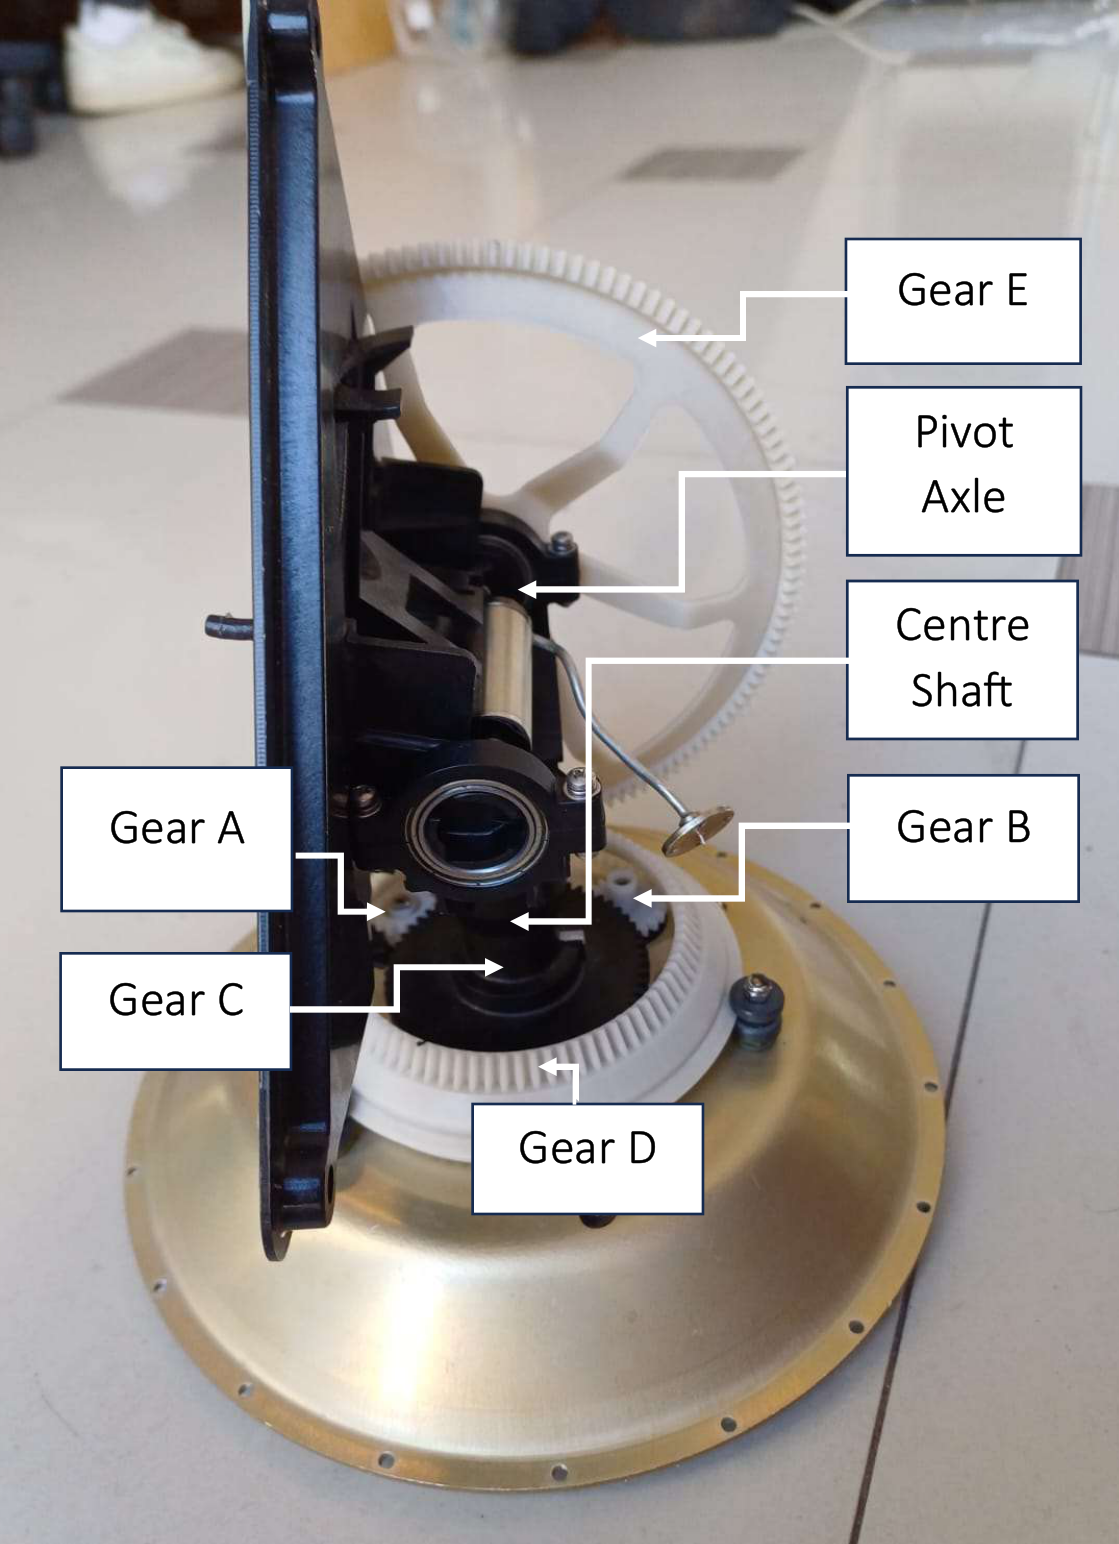
\includegraphics[width=0.4\textwidth]{antennaMount}
    \caption{The Existing Antenna Mount}
    \label{fig:antennaMount}
\end{figure}

Relative orientation can be measured by an inertial measurement unit (IMU), which typically includes an accelerometer and gyroscope. If a magnetometer is included, absolute orientation can also be measured. This will be discussed further in the detailed design stage.

\subsection{Monitoring}
A laptop or PC will be used to monitor the connection. A Graphical User Application (GUI) will be implemented for ease-of-use. This should include the following functionality:
\begin{itemize}
    \item Send specific commands to the satellite.
    \item Read sensor measurements of the satelite.
    \item Control the ground station orientation e.g. performing motor calibration etc.
    \item Set communication parameters e.g. output power and modulation parameters.
    \item Monitor communication link performance.
\end{itemize}